\section*{Results}
The results are separated for registration and segmentation approaches. All were obtained with 20 training images and 10 test images. The results for each case are measured with the Dice score and the Hausdorff distance. They represented with boxplots to show the mean as well as the variability.

\subsection*{Random forest parameters optimization}
For a fixed number of estimator of 10, the random forest approach almost reaches its optimal performance around 20. As the time consumption of the algorithm has not been considered in this work, a margin has been tolerated and the selected number of estimators was 40. 

\begin{figure}[h!]
	\centering
	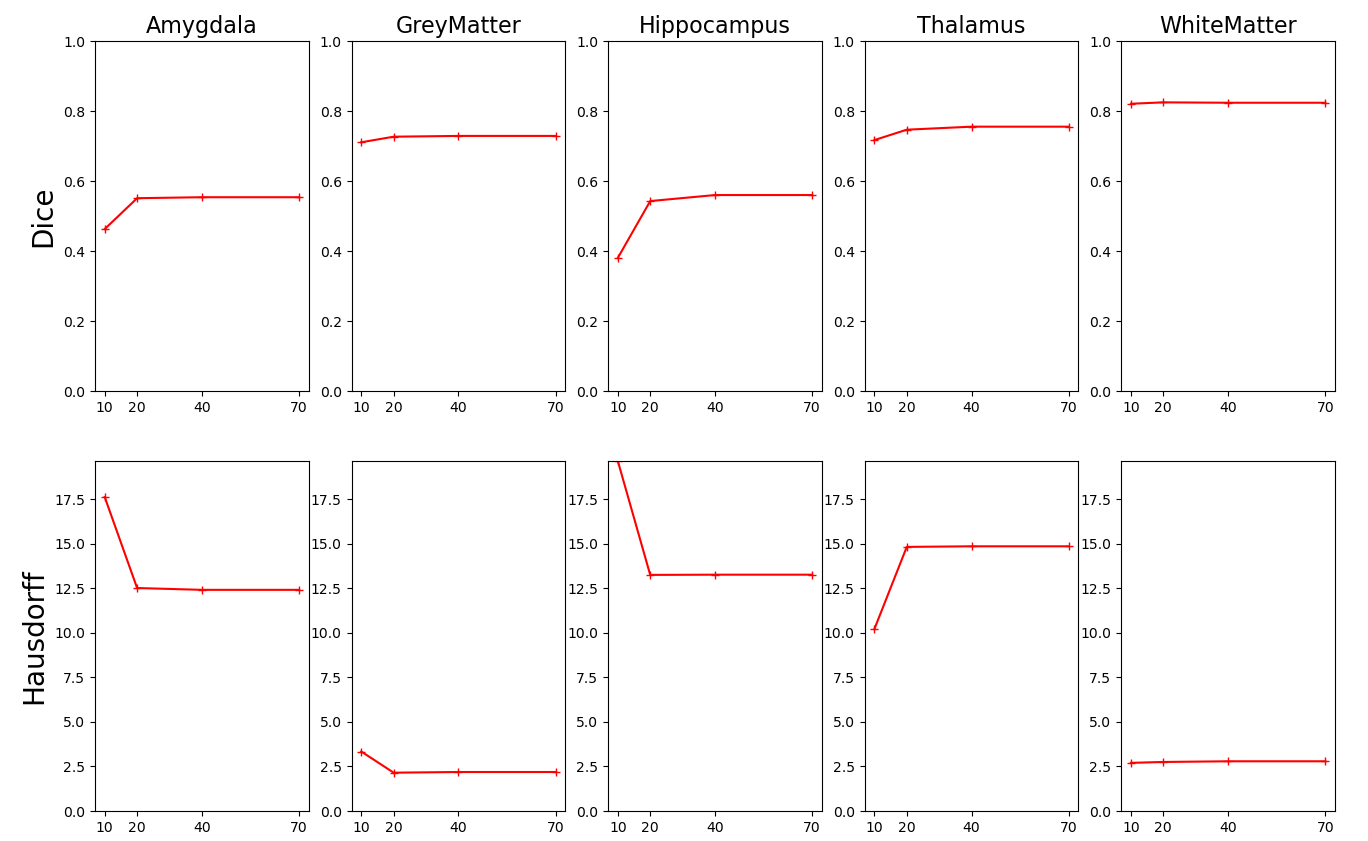
\includegraphics[width=\linewidth]{img/plotMLOptDepth2}
	\caption{Random forest mean Hausdorff distance and dice coefficient for a constant number of estimator of 10.}
	\label{fig:MLOptDepth}
\end{figure}

With a fixed number of estimator, except for the thalamus and hippocampus regions, the random forest shows the best results for a depth of 10. 

\begin{figure}[h!]
	\centering
	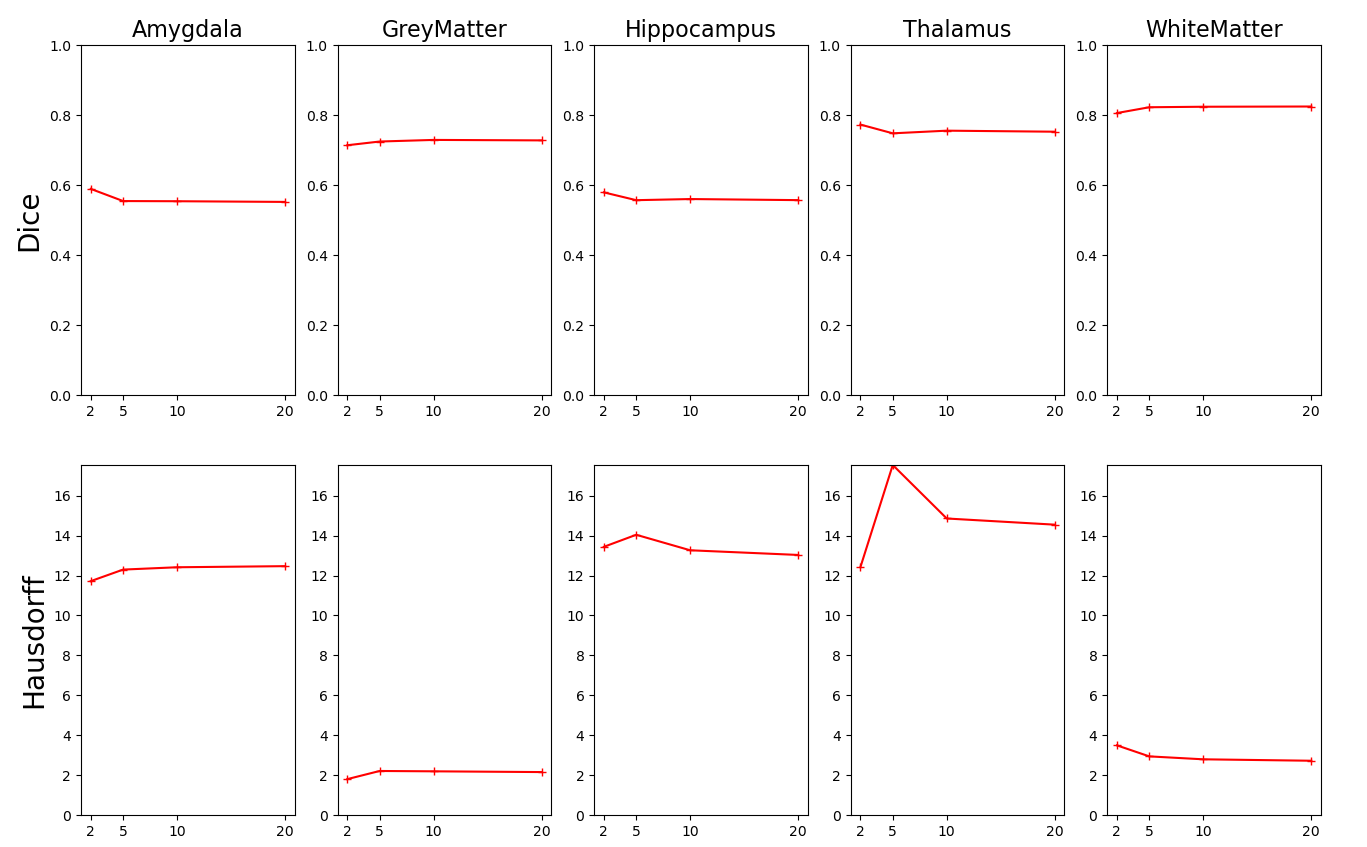
\includegraphics[width=\linewidth]{img/plotMLOptEstimator2}
	\caption{Random forest  mean Hausdorff distance and dice coefficient for a constant depth of 40.}
	\label{fig:MLOptEst}
\end{figure}

\subsection*{Registration}
Two registration methods have been implemented: affine (Aff) and non-rigid (NR). The first is easier to implement and faster to execute, the second one should match the atlas image better as more deformations are possible.

\begin{figure}[h!]
	\centering
	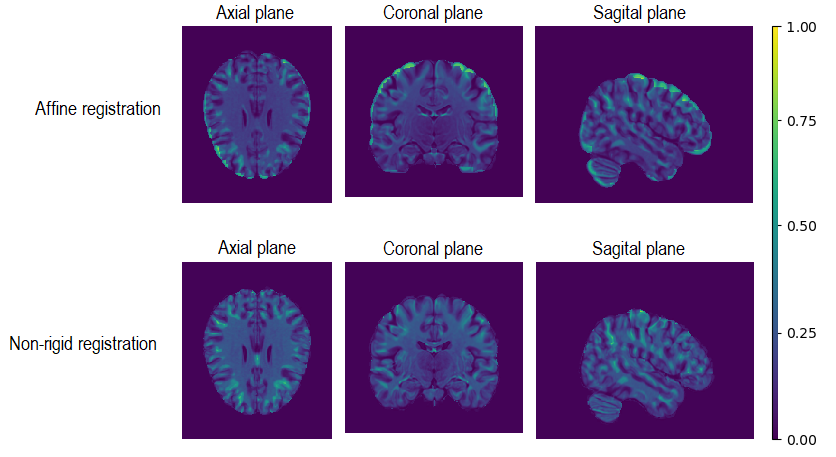
\includegraphics[width=\linewidth]{img/compareRegistration2}
	\caption{Comparison between affine and non-rigid registration by similarity measurement of squared differences of the registered volume to the fixed volume, high values mean larger differences.}
	\label{fig:compareregistration}
\end{figure}

As can be seen in figure \ref{fig:compareregistration} non-rigid registration in the gray matter region is better than affine registration because it can compensate for local changes. What is additionally important is that the non-rigid registration must be reversed after segmentation. Since it does not correspond to the truth.
To compare the effect of the different registration methods, the pipeline was run for both methods with the segmentation methods majority voting (MV) and machine learning (ML). The results of this comparison are represented in figure \ref{fig:boxplotReg}.

\begin{figure}[h!]
	\centering
	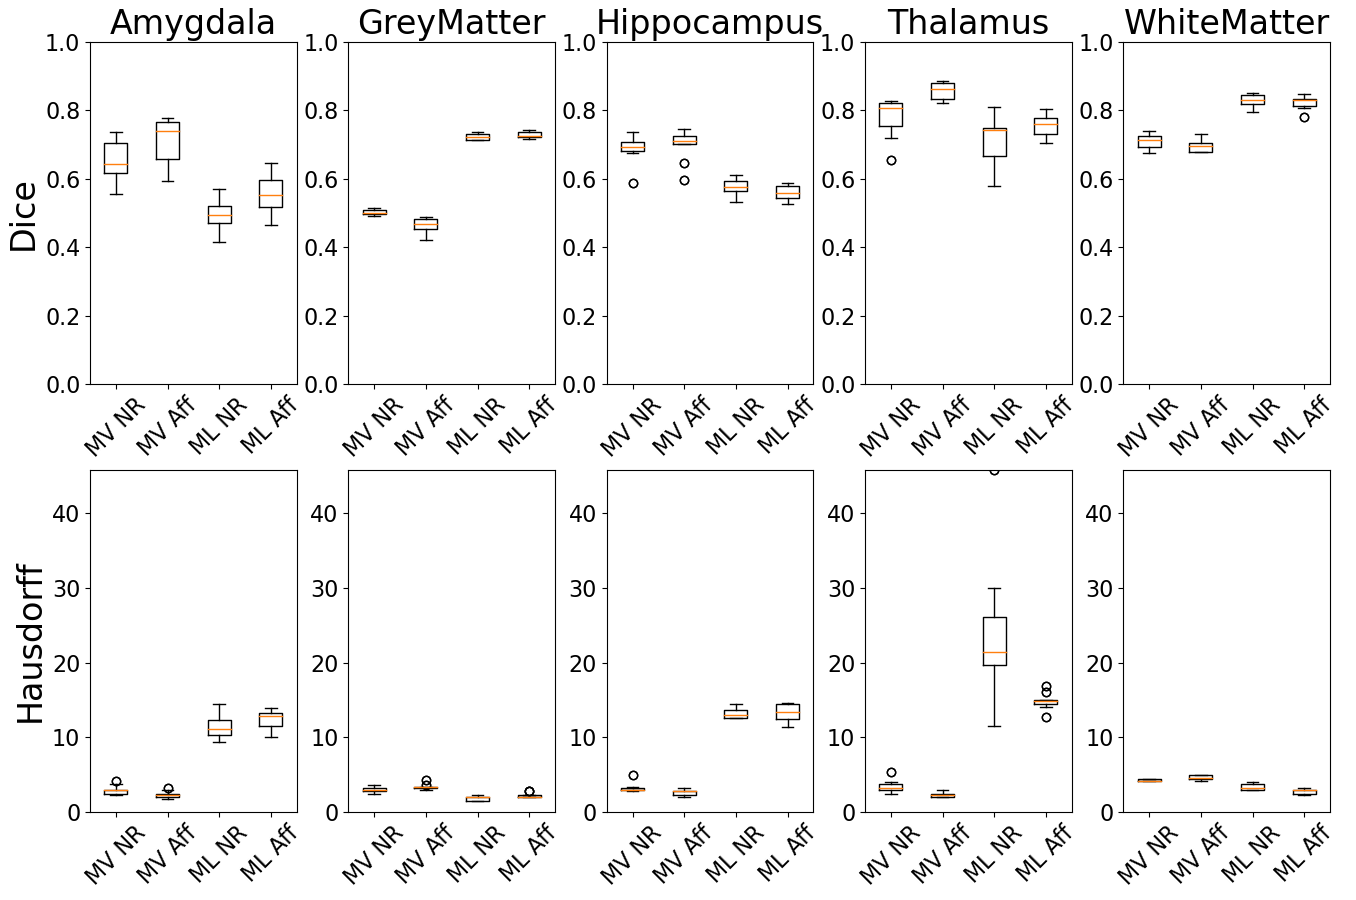
\includegraphics[width = .48 \textwidth]{img/boxplotComparisonNRAff2}
	\caption{Dice and Hausdorff distance result for majority voting (MV) and machine learning (ML) segmentation preceded by non-rigid (NR) or affine (Aff) registration.}
	\label{fig:boxplotReg}
\end{figure}

From the graphic, we can see no clear advantage of the non-rigid registration over the affine one. The difference is too small and has too much variability to choose one registration over the other one.

\subsection*{Segmentation}
Five segmentation methods have been implemented: majority voting (MV), global weighted (GW), local weighted (LW), shape based averaging (SBA) and machine learning (ML). All except the last one are atlas-based. The results with affine registration are represented in the figure \ref{fig:boxplotAff}.

\begin{figure}[h!]
	\centering
	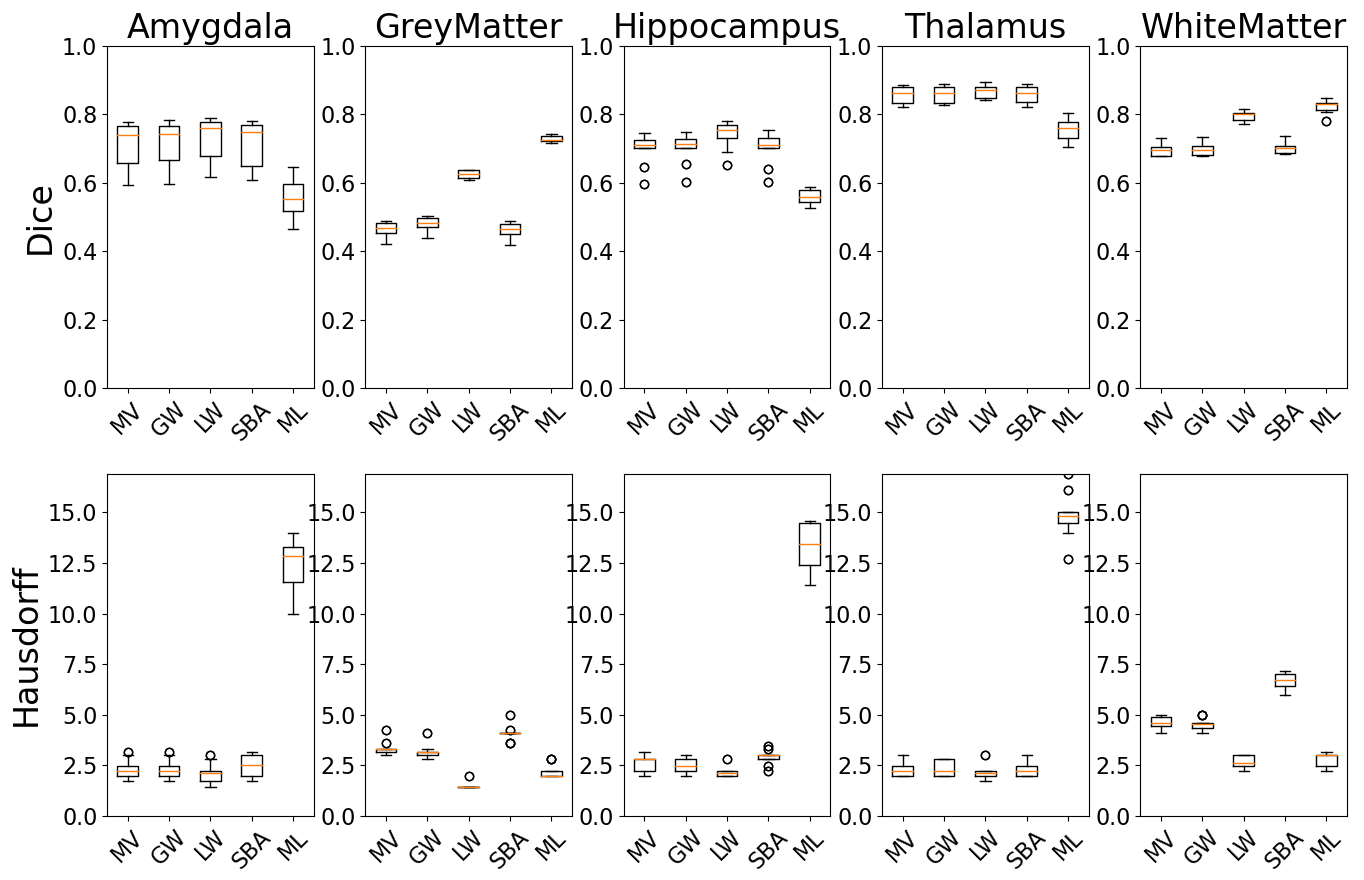
\includegraphics[width = .48 \textwidth]{img/boxplot_Affine_all2}
	\caption{Dice and Hausdorff distance result for majority voting (MV), global weighted (GW), local weighted (LW), shape based averaging (SBA) and machine learning (ML) segmentations preceded by affine registration.}
	\label{fig:boxplotAff}
\end{figure}

For the smaller parts of the brain (Amygdala, Hippocampus and Thalamus), all atlas-based segmentation methods have similar results. Machine learning has more difficulties with those brain parts. On the other hand, it gives better results with grey and white matter. Local weighted atlas significantly performs better than any other atlas-based segmentation methods for those brain parts. It is the best overall segmentation methods.

The same segmentation methods with non-rigid registration are represented in figure \ref{fig:boxplotNR}.

\begin{figure}[h!]
	\centering
	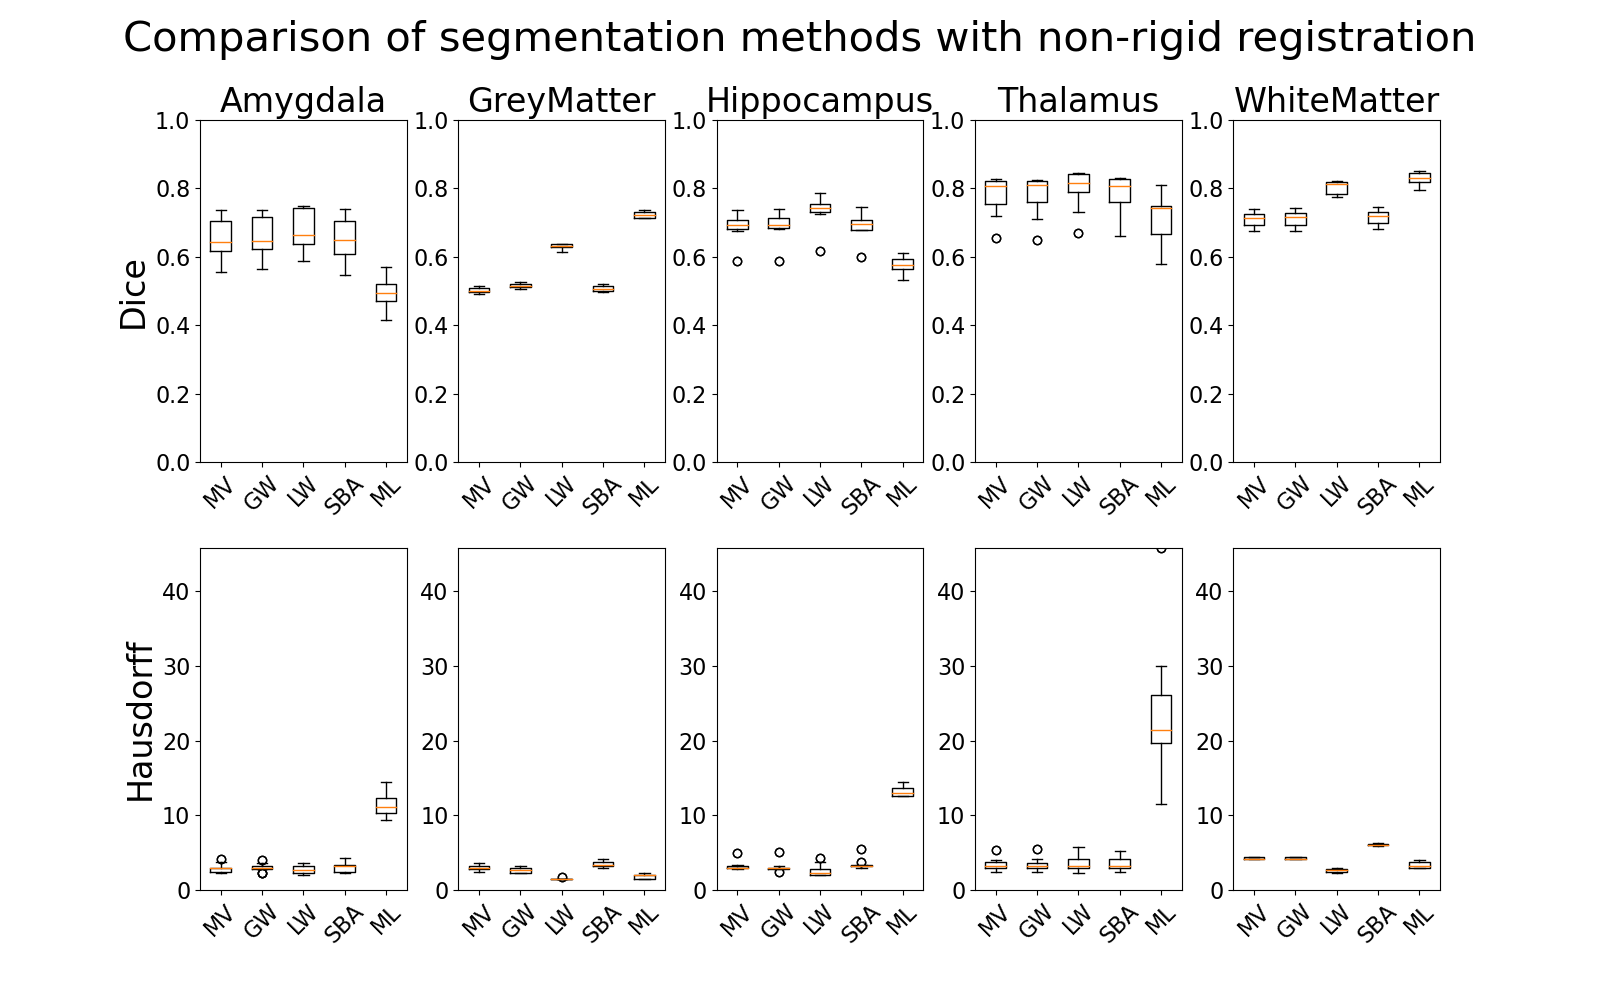
\includegraphics[width = .48 \textwidth]{img/boxplot_NR_all}
	\caption{Dice and Hausdorff distance result for majority voting (MV), global weighted (GW), local weighted (LW), shape based averaging (SBA) and machine learning (ML) segmentations preceded by non-rigid registration.}
	\label{fig:boxplotNR}
\end{figure}

In general, the results are very similar to the one with affine registration. Machine learning seems to struggle even more with the Thalamus, as the Hausdorff distance suggests.
